\documentclass[10pt,letterpaper]{article}
\usepackage[utf8]{inputenc}
\usepackage[english]{babel}
\usepackage{indentfirst}
\usepackage{titlesec}
\usepackage{graphicx}
\usepackage[super]{nth}
\usepackage{amsmath}
\usepackage{amsfonts}
\usepackage{amssymb}
\usepackage{geometry}
\usepackage{float}
\usepackage{titlesec}
\usepackage{lipsum}
\titlespacing\section{0pt}{6pt plus 4pt minus 2pt}{0pt plus 2pt minus 2pt}
\titlespacing\subsection{0pt}{4pt plus 2pt minus 2pt}{0pt plus 2pt minus 2pt}

\setlength{\parskip}{\baselineskip}%
\setlength{\parindent}{0pt}%
 \geometry{
 a4paper,
 total={170mm,260mm},
 left=20mm,
 top=15mm,}

\begin{document}
\begin{titlepage}
    \begin{center}
        \vspace*{10cm}
 
        \Huge
        \textbf{ECE1513: Machine Learning Project}
 
        \vspace{0.5cm}
        \LARGE
        How does an NHL Playoff Team Look
 
        \vspace{1.5cm}
 
        \textbf{Omar Ismail}
 
        \vfill
 

 
        \vspace{0.8cm}
 

        \Large
        University of Toronto\\
        April 2019
 
    \end{center}
\end{titlepage}


\section*{Introduction}
The excitement level of millions of people rises each October as the NHL season begins. 31 teams, each playing 82 games, with the top teams qualifying to the Stanley Cup playoffs. The NHL is split into 2 conferences, East and West, with each conference further split into 2 Divisions. 8 teams from each conference qualify for the playoffs: the top 3 teams in each division, plus 2  "wild card" teams from each conference. These wild card teams are the ones that finish \nth{7} and \nth{8} in their conference. Can we use previous years data to predict which teams should be in the playoffs this year? This is the question we are trying to answer. As of writing this report, the regular season has ended, so we can compare our machine-learned predictions to reality. 

\section*{Making the Dataset}
The first step is making the dataset. We will use historical data starting from the salary cap era (2005). Even though the NHL has been in existence since 1917, prior to 2005, there was no restriction on the amount of spending on players. With the enforcement of a salary cap, the playing field became more level.  The data was collected from [1], and for each of the 391 teams, a 0 is assigned if the team made the playoffs that season, and 1 otherwise. The data consists of 33 features. As our dataset is not large and we have a lot of features, we want to avoid over-fitting. To do so, we need to cut down the number of features.    
\subsection*{Feature Selection}
We want to be able to predict a playoff team without knowing the team's ranking, or factors that influence ranking, as that would make the task trivial. So, we got rid of these features. These are:
\begin{itemize}
    \item Ranking and Games Played
    \item Wins and Losses (which include overtime and shootouts) 
    \item Strength of Schedule (this looks at strength of opponents)
    \item Simple Rating System (this determines how good a team is)
\end{itemize}

We also make sure we do not have repetitive features. For example, there is a Goals Scored feature, but also Even Strength Goals Scored, as well as Power Play Goals Scored, the summation of the latter two giving the former. So we removed the former. The result is that we are able to reduce our features from 33 to 19. We would like to further reduce our features. We found that the Random Forest Classifier has a tool which is able to identify the important features. We use this to identify the Top 3 features. A visualization is shown below:
\begin{figure}[H]
    \centering
    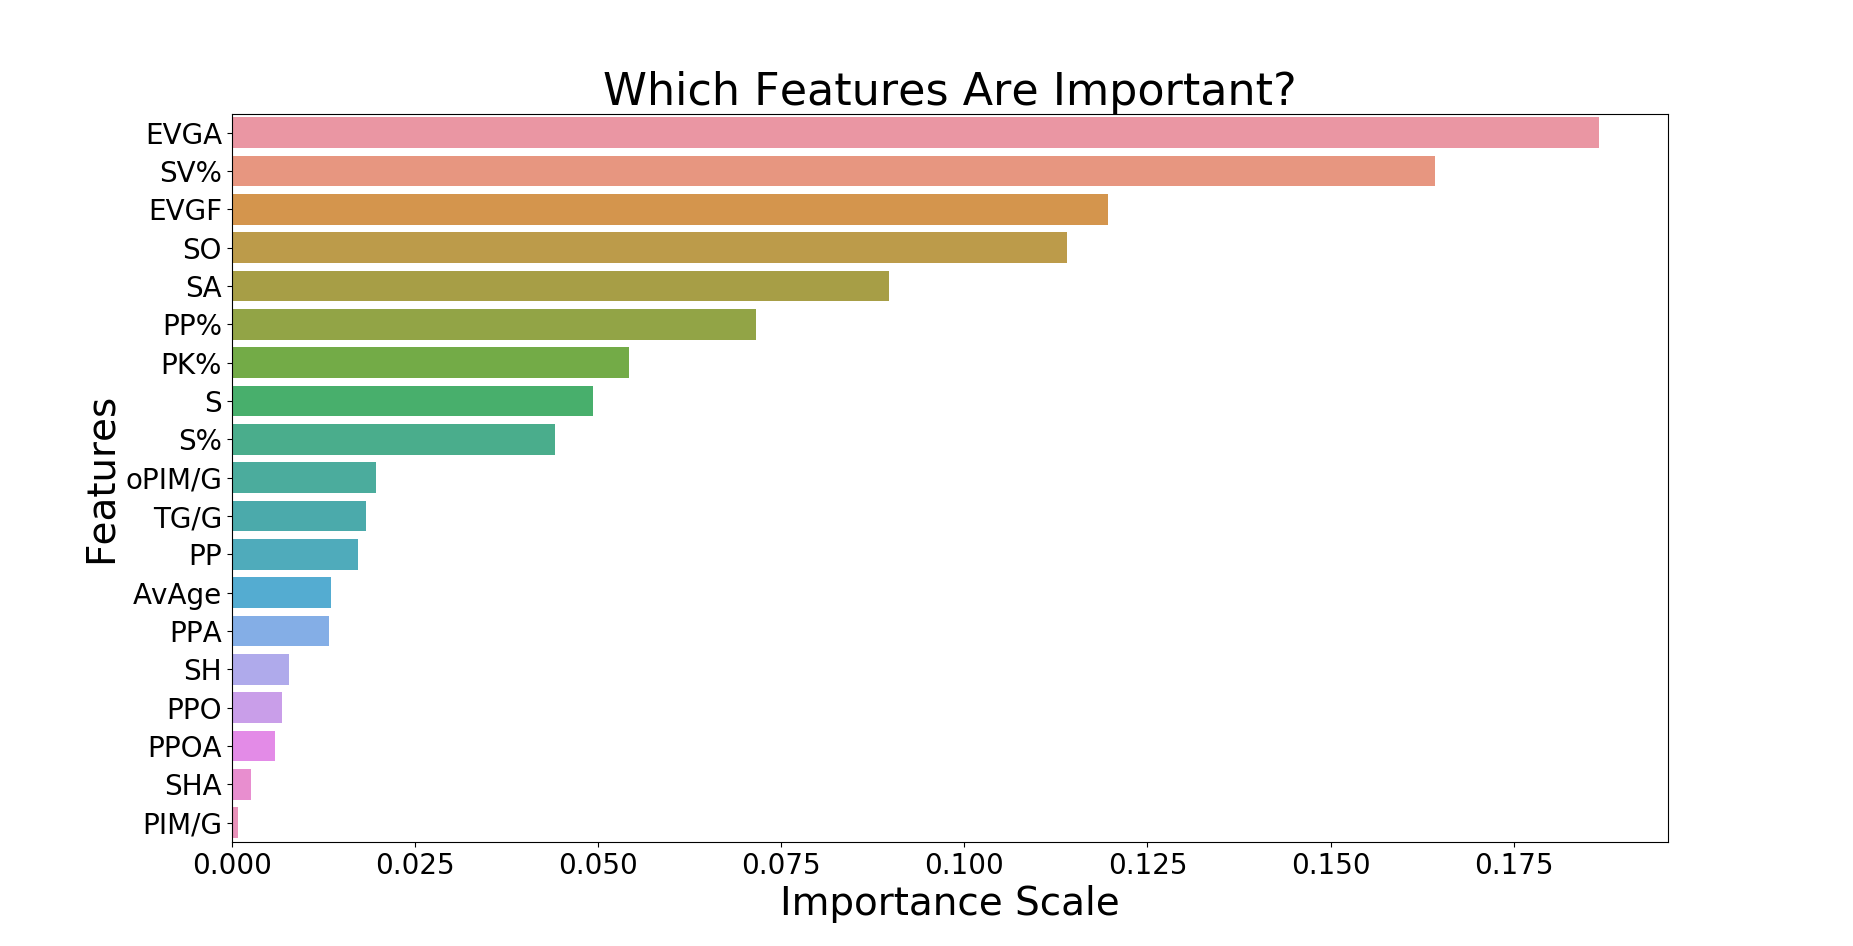
\includegraphics[scale = 0.25]{Important.png}
    \caption{Feature Selection}
    \label{fig:feature}
\end{figure}
As seen in Figure \ref{fig:feature}, the top 3 features are  Even Strength Goals Against (EVGA), Goalie Save Percentage (SV\%), and Even Strength Goals For(EVGF). These 3 features are the ones we will use going forward. Note, that the code has the capability of choosing more than 3 features.

\section*{Using K-Means to Classify}
In this section we use K-Means to see if we can distinguish between playoff and non-playoff teams based on the 3 features selected (EVGA, EVGF, and SV\%); thus, our K value is 2. To assess the accuracy of the clustered points, we will compare the assigned points to each cluster to the actual targets for both training and validation sets. We then look at how this year's teams cluster using K-Means and comment on how accurate that is. 

\subsection*{Results and Discussion}
First, we show our training and validation set plots in the figure below. We can see that after around 70 epochs, the validation set loss starts to increase, so we stop the training their:
\begin{figure}[H]
    \centering
    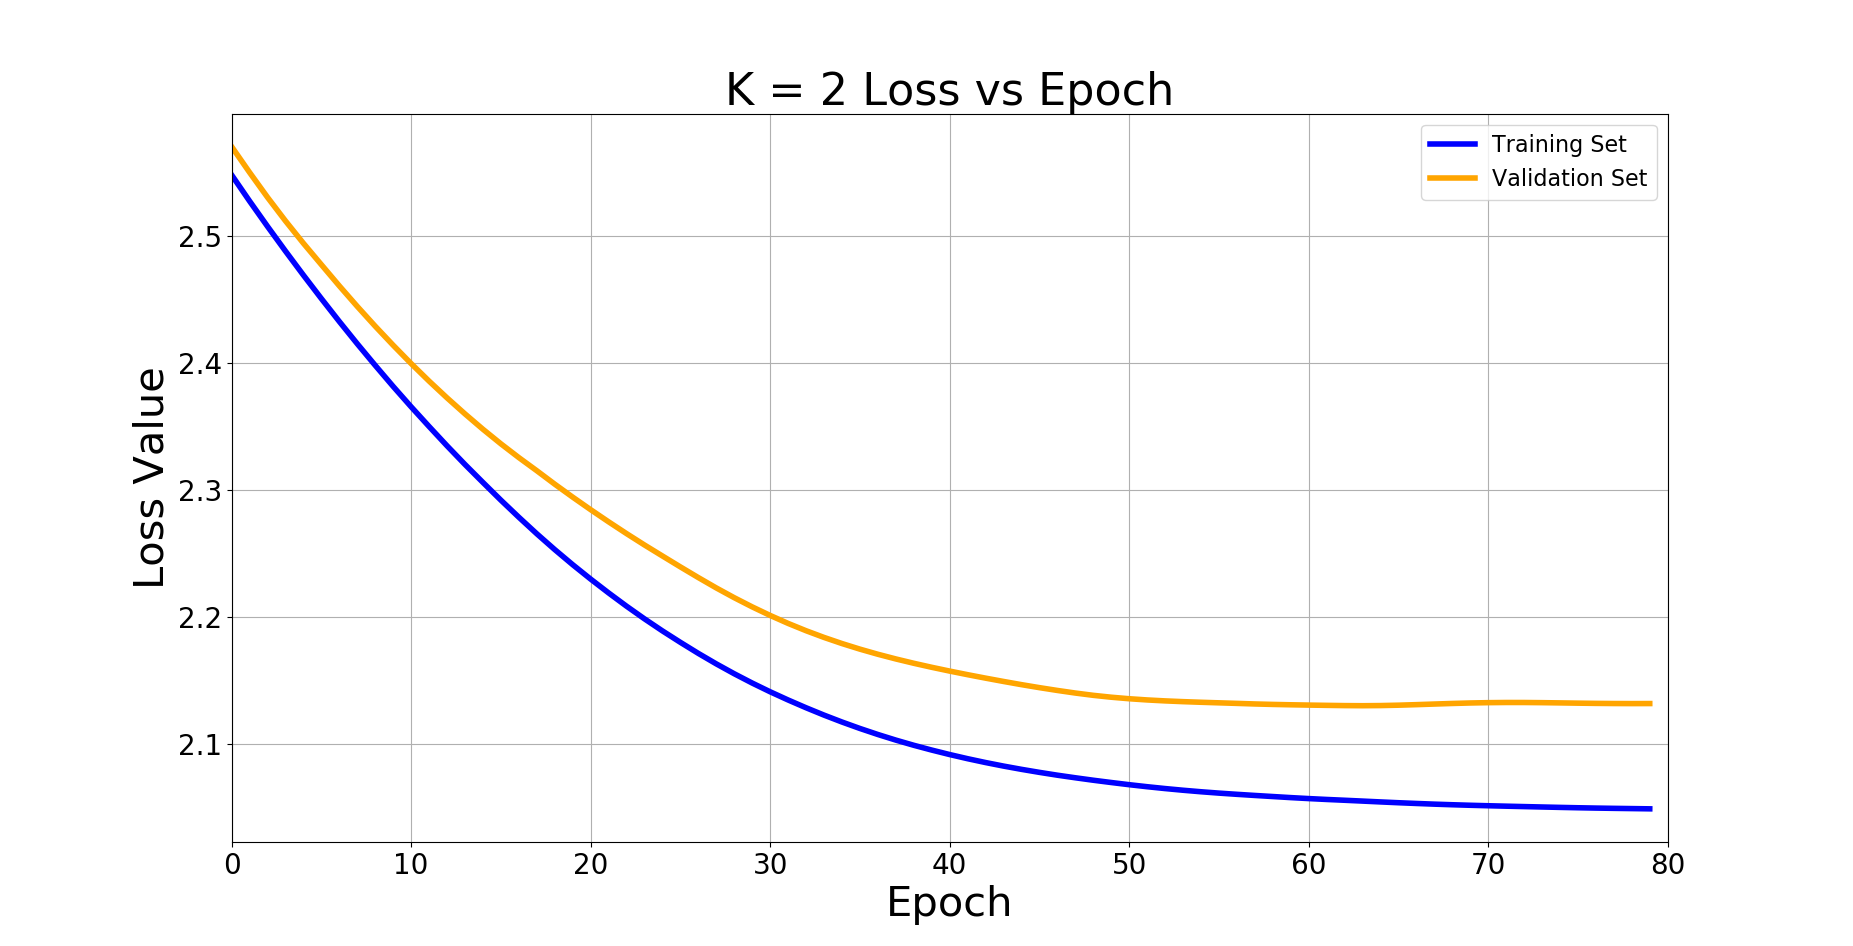
\includegraphics[scale = 0.23]{kLoss.png}
    \caption{Training and Validation Set Loss vs Number of Epochs}
    \label{fig: kLoss}
\end{figure}

When we compared the accuracy of this model to the actual data of previous years, we found the clustering algorithm was 67\% accurate on both training and validation sets. This may seem low, but an argument can be made that it is reasonable. The accuracy numbers can be interpreted as: using statistics on just the goals scored, goals against, and goalie save percentage, we are able to determine if a team is a playoff team 67\% of the time. In the real-world, there are many more factors that influence if a team makes the playoffs, including luck; however, these models can be very difficult to formulate. 

You might ask why not use more or less features, as opposed to just 3. We tried this for different feature set sizes: 2, 4, 8, and all of them, and found the training set accuracy for each feature was 27\%, 21\%, 20\%, 32\%  respectively, which is considerably less than when the feature size is 3.

Let's look at how K-Means clustered this year's teams, where red identifies teams in playoffs, and blue otherwise:
\begin{figure}[H]
    \centering
    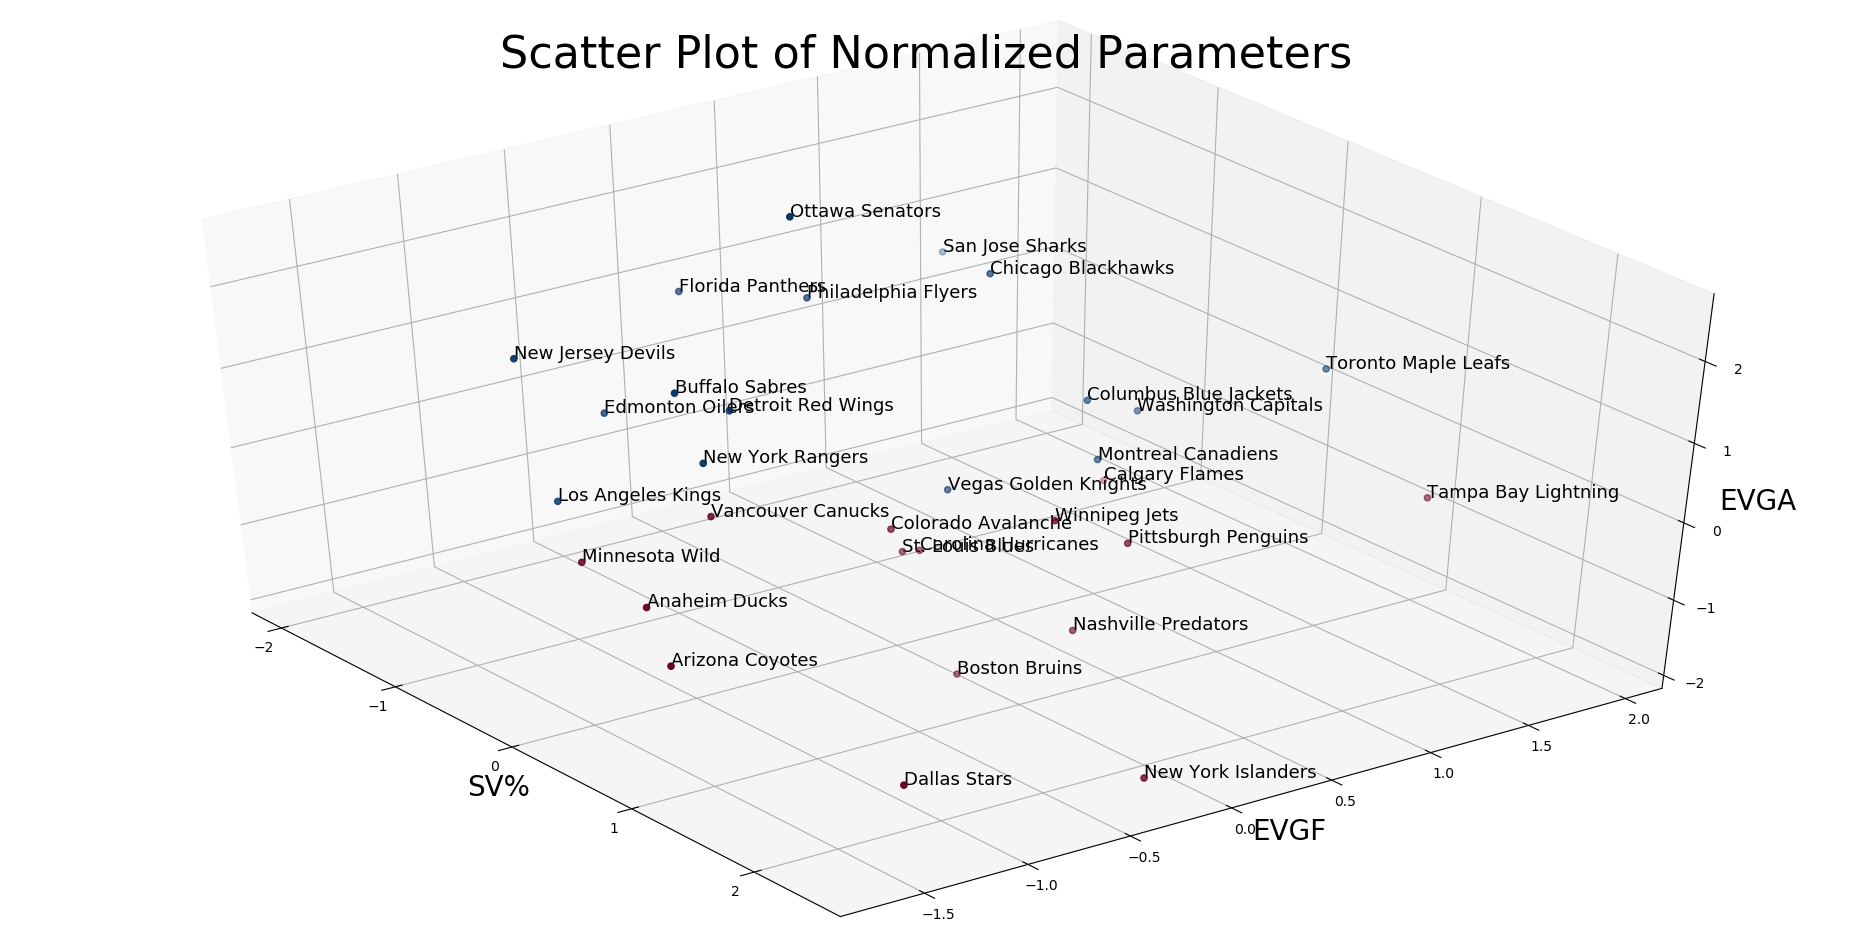
\includegraphics[scale = 0.3]{kScatter.png}
    \caption{Who is making the playoffs according to K-Means Clustering}
    \label{fig:my_label}
\end{figure}

Some observations:
\begin{itemize}
    \item It identified 15 teams making the playoffs, this is one short of what, where 16 teams make the playoffs
    \item You can easily see the difference in the plot between the best teams in the league, like the Tampa Bay Lightning, and the worst, the Ottawa Senators
    \item Out of the 15 predicted playoff teams, 4 of them did not and they all are in the same area: Vancouver, Minnesota, Anaheim and Phoenix. The area they are in is where they have better than league-average goaltending, but much worse scoring.
    \item Out of the 16 predicted non-playoff teams, 5 of them actually made it: Toronto, Columbus, Vegas,  Washington and San Jose. The outlier here seems to be San Jose, who have one of the worse goaltending save percentages in the league, but make up for that by being on the higher end of scoring, and playing in the weakest division this year: the Pacific. 
    \item With 9 incorrect predictions, the accuracy of the model on this year's data is 71\%, which is close to the training and validation accuracies
\end{itemize}


\section*{Using Logistic Regression}
In this section and the next, we factor into our training and validation data whether a team made the playoffs, therefore we move from unsupervised to supervised learning. The first supervised algorithm we will use is Logistic. Our model is as follows:
\begin{align*}
    \sigma (x^TW+b)
\end{align*}
In this model, the outputted vector is the probability of a team \textbf{not} making the playoffs. We use the Adam Optimizer to find the weights and biases that minimize the model above, and add a regularization term of 0.01 to avoid over-fitting the data.

\subsection*{Results and Discussion}
The loss and accuracy plots on the training and validation data is shown below:
\begin{figure}[H]
    \centering
    \includegraphics[scale = 0.25]{logLA.png}
    \caption{Logistic Regression Loss and Accuracy Plots}
    \label{fig:Logistic}
\end{figure}
The noise in the training set is likely due to the small batch size 13, and the small training set size, 312 points. The final training and validation set accuracy are 100\% and 84.8\%. Our final weight and bias vectors are:
\begin{align*}
    W = \begin{bmatrix}
           -0.66 \\
           -1.67 \\
            1.75
         \end{bmatrix} \text{,                 }
   b = \begin{bmatrix}
   -0.13
 \end{bmatrix}  
\end{align*}

Using these values we can calculate the probability of each team making the playoffs. Unlike unsupervised learning were the algorithm only divides teams into 0 or 1, the logistic gives us a range between these two values. The model allows us to always choose the right number of playoff teams. Not only can this model predict the playoff bound teams, but it can also predict the first-round match-ups in the play-offs. For this year, the predicted playoff match-ups are as follows:
\begin{align*}
    \textbf{Eastern Conference Match-ups:}\\
    \text{1. Tampa Bay Lightning } &\text{vs. } \text{WC2. Carolina Hurricanes}\\
    \text{2. Boston Bruins } &\text{vs. } \text{3. Toronto Maple Leafs}\\
    \text{1. New York Islanders } &\text{vs. } \text{WC1. Montreal Canadiens}\\
    \text{2. Pittsburgh Penguins } &\text{vs. } \text{3. Washington Capitals}\\
    \textbf{Western Conference Matchups:}\\
    \text{1. Calgary Flames } &\text{vs. } \text{WC2. Colorado Avalanche}\\
    \text{2. Vegas Golden Knights } &\text{vs. } \text{3. San Jose Sharks}\\
    \text{1. Nashville Predators } &\text{vs. } \text{WC1. Winnipeg Jets}\\
    \text{2. Dallas Stars } &\text{vs. } \text{3. St. Louis Blues}
\end{align*}


Apart from the Canadiens, every team predicted to make the playoffs matched reality! The Columbus Blue Jackets made it instead. So the predictor got 2 teams wrong, yeilding an accuracy of 92.3\%. It might seem like Montreal got really unlucky this year; looking at the figure below, it seems the logistic predictor had them as the first Wild Card team. Of note is how the model does well in segmenting the teams that had no chance towards the end of the season in making the playoffs from teams that were in the hunt for a spot; towards the end of the season, the last 2 playoff spots was contested tightly between Montreal, Carolina, and Columbus.
\begin{figure}[H]
    \centering
    \includegraphics[scale= 0.45]{unlucky.png}
    \caption{Wild Card East Race}
    \label{fig:WCE}
\end{figure}
In terms of predicted first round match-ups, only 3 of the match-ups were predicted correctly: Boston vs Toronto, Calgary vs Colorado, and Vegas vs San Jose. From these, just 1 had the seeding incorrect: Vegas vs San Jose. 



\section*{Using Neural Network to Classify}
Now we look at a more complicated supervised learning algorithm: a Neural Net. We implement a 3-layer MLP, with a drop-out layer between the \nth{2} and the \nth{3} layer. The hidden unit layers each have 500 nodes. The drop-out rate is set to 0.5, and just like in logistic regression, the regularization is set to 0.01.
\subsection*{Results and Discussion}
The loss and accuracy plots are shown below:
\begin{figure}[H]
 	\centering
    \includegraphics[scale= 0.25]{netLA.png}
    \caption{Neural Net Loss and Accuracy Plots}
    \label{fig:Neural}
\end{figure}

The final training and validation set accuracy are 100\% and 83.5\%. Note that the validation accuracy is 1\% less than logistic regression, which is a minor change. It may seem like extending the classification of the dataset to a more complicated alogrithm did not make a difference. Using this neural net, the predicted playoff match-ups are as follows:
\begin{align*}
    \textbf{Eastern Conference Match-ups:}\\
    \text{1. Tampa Bay Lightning } &\text{vs. } \text{WC2. Carolina Hurricanes}\\
    \text{2. Boston Bruins } &\text{vs. } \text{3. Toronto Maple Leafs}\\
    \text{1. New York Islanders } &\text{vs. } \text{WC1. Montreal Canadiens}\\
    \text{2. Pittsburgh Penguins } &\text{vs. } \text{3. Washington Capitals}\\
    \textbf{Western Conference Matchups:}\\
    \text{1. Calgary Flames } &\text{vs. } \text{WC2. Colorado Avalanche}\\
    \text{2. Vegas Golden Knights } &\text{vs. } \text{3. San Jose Sharks}\\
    \text{1. Nashville Predators } &\text{vs. } \text{WC1. Dallas Stars}\\
    \text{2. St. Louis Blues } &\text{vs. } \text{3. Winnipeg Jets}
\end{align*}


Again, the model misclassifies Montreal and Columbus, yeilding an accuracy of 92.3\%, the same as the simpler logistic model. In terms of predicted first round match-ups,  5 of the match-ups were predicted correctly: Boston vs Toronto, and the entire Western Conference. From these, just 2 had the seeding incorrect: Vegas vs San Jose, and Winnipeg vs St. Louis. Note that Winnipeg and St. Louis finished with the same amount of points this year, but the tie-breaker for the higher seed went to Winnipeg!

\section*{Conclusion}
It seems like the added complexity of the neural net model only imporves predicting the first-round match-ups compared to the logistic model. In terms of predicting the correct teams making the playoffs, both models return the same results. This makes sense: a neural nets advantage of being a non-linear classifier shows when we got a very large dataset. In th 






\end{document}
